\subsection{Setup 3 - Agglomerative: Resultados nos Datasets Adult e Dry Bean}

Neste setup, avaliamos o desempenho do Agglomerative Clustering supervisionado nos conjuntos Adult (balanceado) e Dry Bean (balanceado), ambos após pré-processamento e balanceamento por oversampling. O pipeline seguiu as etapas de normalização, divisão estratificada, definição do número de clusters (via método do cotovelo/silhouette), treinamento, repetição dos experimentos (30 execuções) e análise quantitativa.

\subsubsection{Adult (Balanceado)}

O Agglomerative foi executado com $n_{clusters}=8$, conforme sugerido pelo método do cotovelo (silhouette). Os resultados médios das 30 repetições estão na Tabela~\ref{tab:agglo_adult_metrics}.

% Tabela Adult apenas acurácia e desvio padrão
\begin{table}[H]
\centering
\caption{Resultados quantitativos do Agglomerative no dataset Adult (balanceado, $n_{clusters}=8$)}
\label{tab:agglo_adult_metrics}
\begin{tabular}{lcc}
\toprule
Métrica & Média & Desvio Padrão \\
\midrule
Acurácia & 0.6932 & 0.0148 \\
\bottomrule
\end{tabular}
\end{table}

As principais visualizações estão apresentadas a seguir:
\begin{figure}[ht]
    \centering
    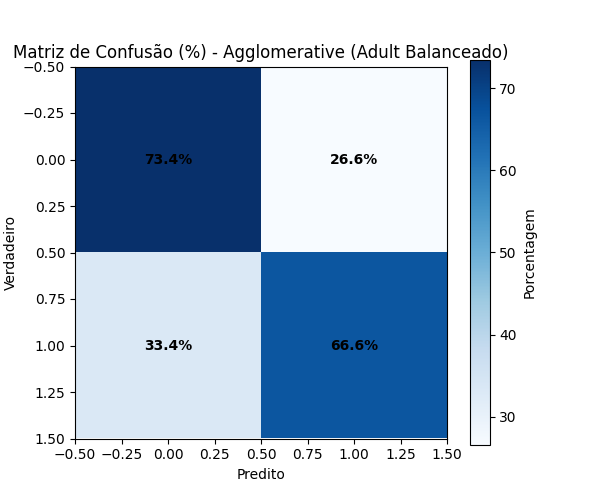
\includegraphics[width=0.7\linewidth]{../src/img/agglo_adult_balance_confusion_matrix.png}
    \caption{Matriz de confusão (Agglomerative - Adult Balanceado)}
    \label{fig:agglo_adult_balance_confusion_matrix}
\end{figure}

\begin{figure}[ht]
    \centering
    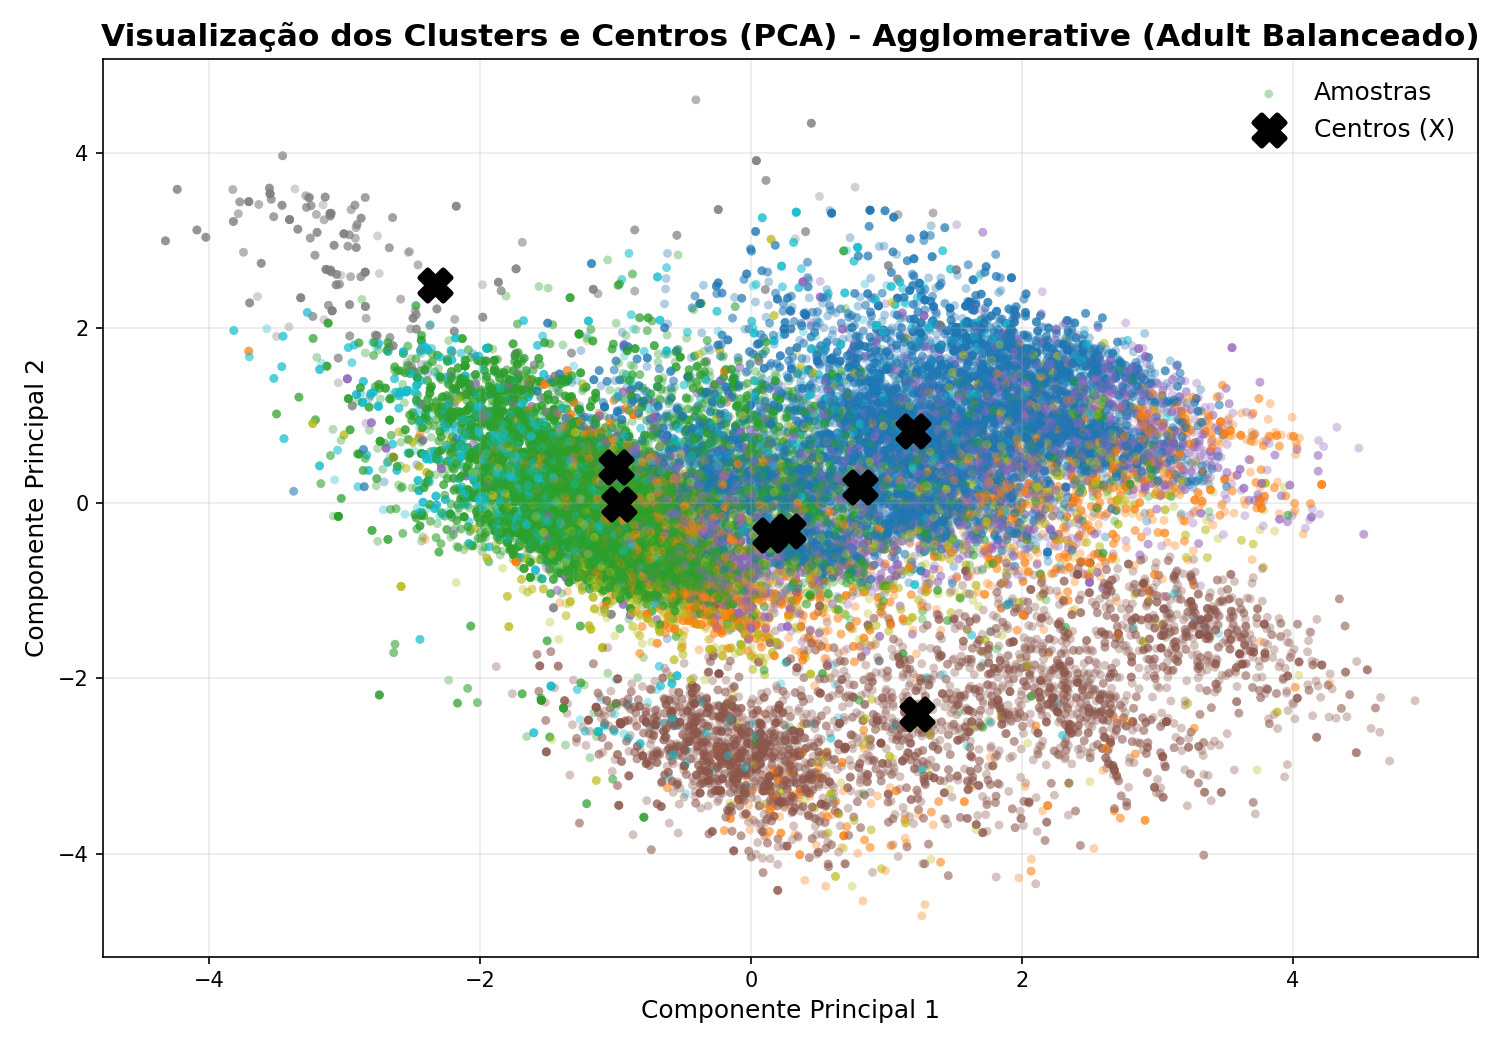
\includegraphics[width=0.7\linewidth]{../src/img/agglo_adult_balance_clusters_pca.png}
    \caption{Visualização PCA dos clusters e centros (Agglomerative - Adult Balanceado)}
    \label{fig:agglo_adult_balance_clusters_pca}
\end{figure}

\begin{figure}[ht]
    \centering
    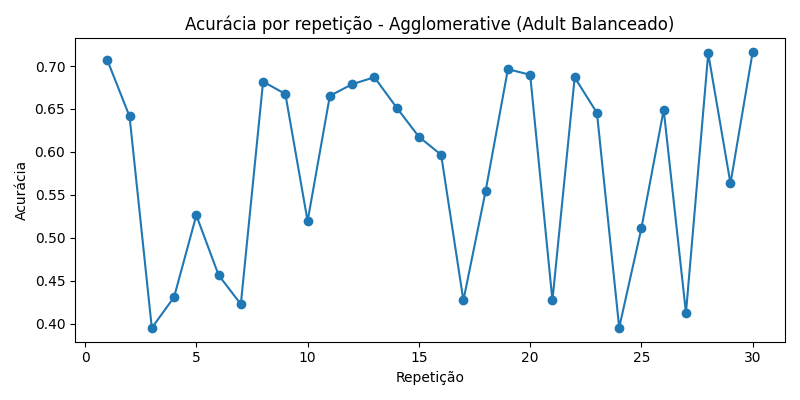
\includegraphics[width=0.7\linewidth]{../src/img/agglo_adult_balance_accuracy_repetitions.png}
    \caption{Acurácia por repetição (Agglomerative - Adult Balanceado)}
\end{figure}

% \begin{figure}[ht]
%     \centering
%     \includegraphics[width=0.7\linewidth]{../src/img/agglo_adult_balance_silhouette.png}
%     \caption{Silhouette médio por número de clusters (Agglomerative - Adult Balanceado)}
% \end{figure}

\subsubsection{Adult: Amostras e Pré-processamento}

O conjunto Adult possui 48.842 amostras, 14 atributos e 2 classes (renda). O pré-processamento incluiu normalização e codificação de variáveis categóricas. O balanceamento foi realizado por oversampling.

\begin{figure}[ht]
    \centering
    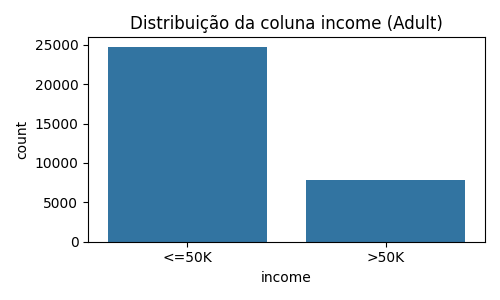
\includegraphics[width=0.7\linewidth]{../src/img/adult_income_hist_before_balance.png}
    \caption{Distribuição das classes no Adult antes do balanceamento}
    \label{fig:adult_hist_before_balance}
\end{figure}

\begin{figure}[ht]
    \centering
    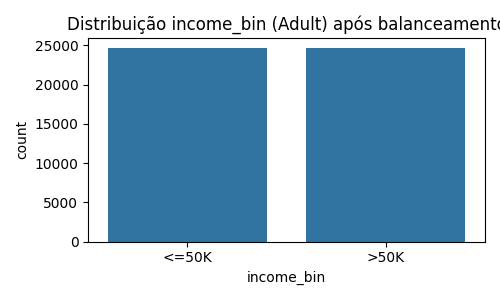
\includegraphics[width=0.7\linewidth]{../src/img/adult_income_hist_after_balance.png}
    \caption{Distribuição das classes no Adult após o balanceamento}
    \label{fig:adult_hist_after_balance}
\end{figure}

\subsubsection{Dry Bean (Balanceado)}

No dataset Dry Bean, o Agglomerative foi executado com $n_{clusters}=7$ e 30 repetições, conforme sugerido pelo método do cotovelo (silhouette). Os resultados estão sumarizados na Tabela~\ref{tab:agglo_drybean_metrics}.

% Tabela Dry Bean apenas acurácia e desvio padrão
\begin{table}[H]
\centering
\caption{Resultados quantitativos do Agglomerative no dataset Dry Bean (balanceado, $n_{clusters}=7$)}
\label{tab:agglo_drybean_metrics}
\begin{tabular}{lcc}
\toprule
Métrica & Média & Desvio Padrão \\
\midrule
Acurácia & 0.6125 & 0.0112 \\
\bottomrule
\end{tabular}
\end{table}

As principais visualizações estão apresentadas a seguir:
\begin{figure}[ht]
    \centering
    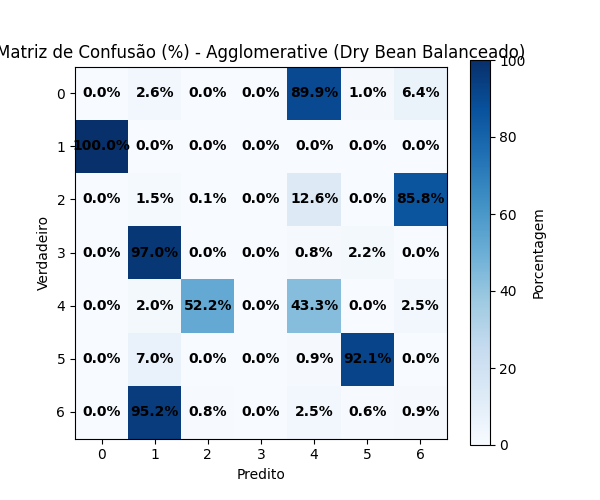
\includegraphics[width=0.7\linewidth]{../src/img/agglo_drybean_balance_confusion_matrix.png}
    \caption{Matriz de confusão (Agglomerative - Dry Bean Balanceado)}
    \label{fig:agglo_drybean_balance_confusion_matrix}
\end{figure}

\begin{figure}[ht]
    \centering
    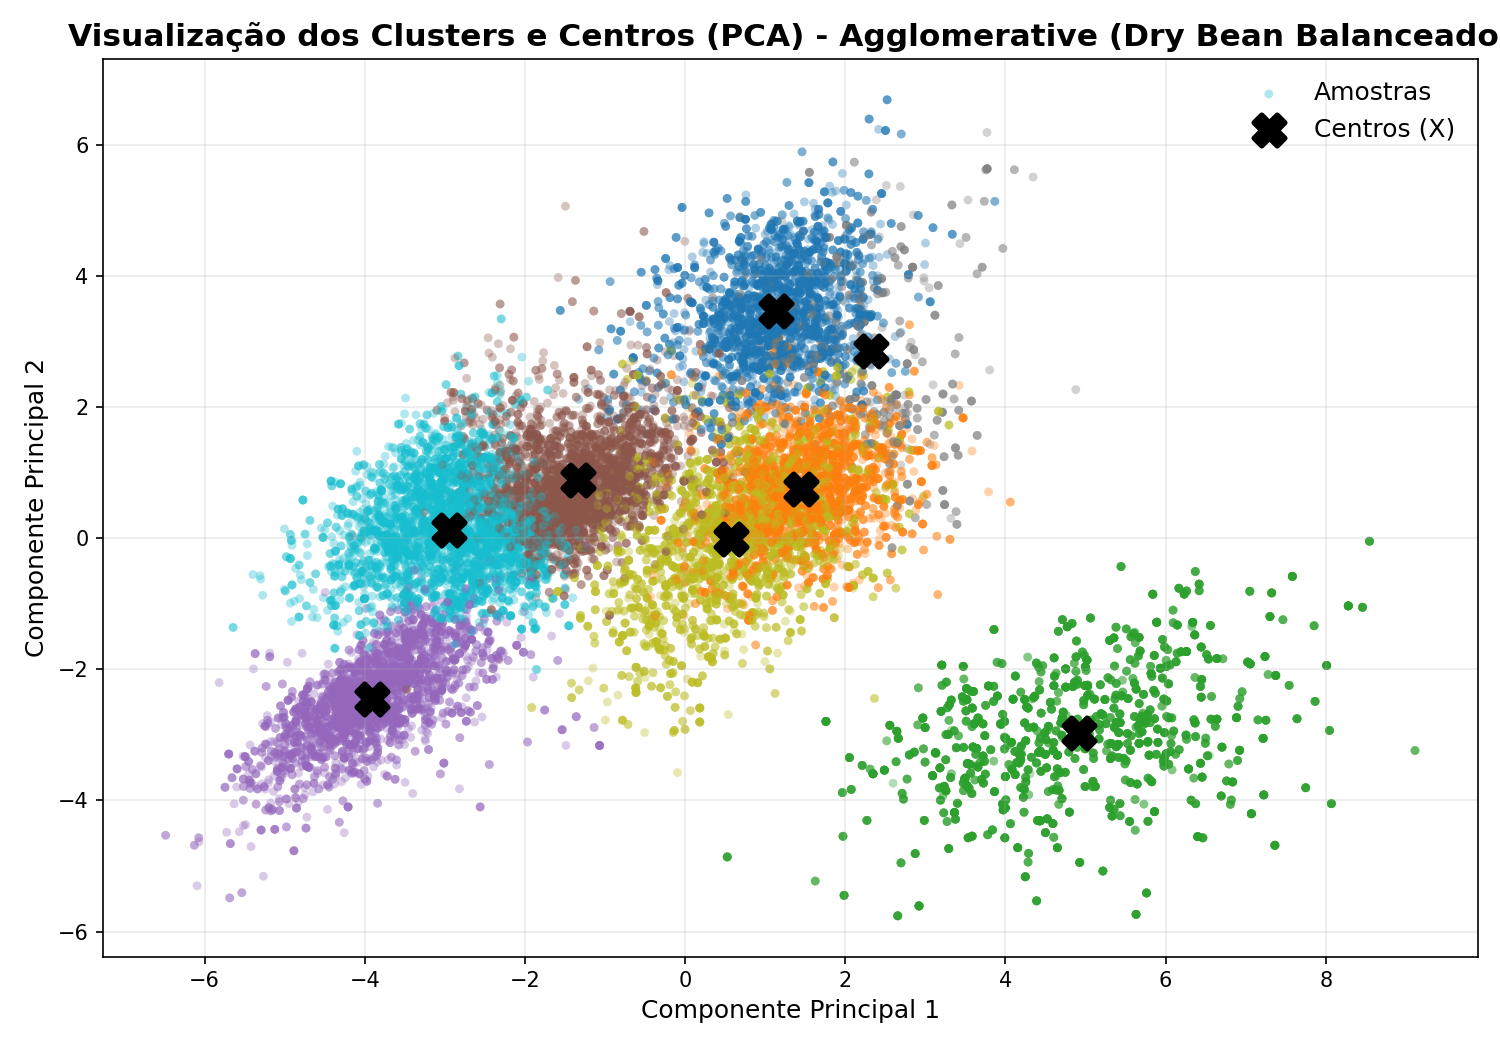
\includegraphics[width=0.7\linewidth]{../src/img/agglo_drybean_balance_clusters_pca.png}
    \caption{Visualização PCA dos clusters e centros (Agglomerative - Dry Bean Balanceado)}
    \label{fig:agglo_drybean_balance_clusters_pca}
\end{figure}

\begin{figure}[ht]
    \centering
    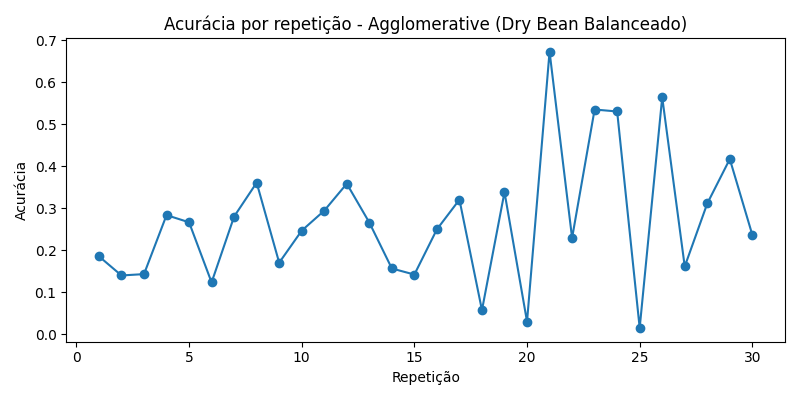
\includegraphics[width=0.7\linewidth]{../src/img/agglo_drybean_balance_accuracy_repetitions.png}
    \caption{Acurácia por repetição (Agglomerative - Dry Bean Balanceado)}
\end{figure}

\begin{figure}[ht]
    \centering
    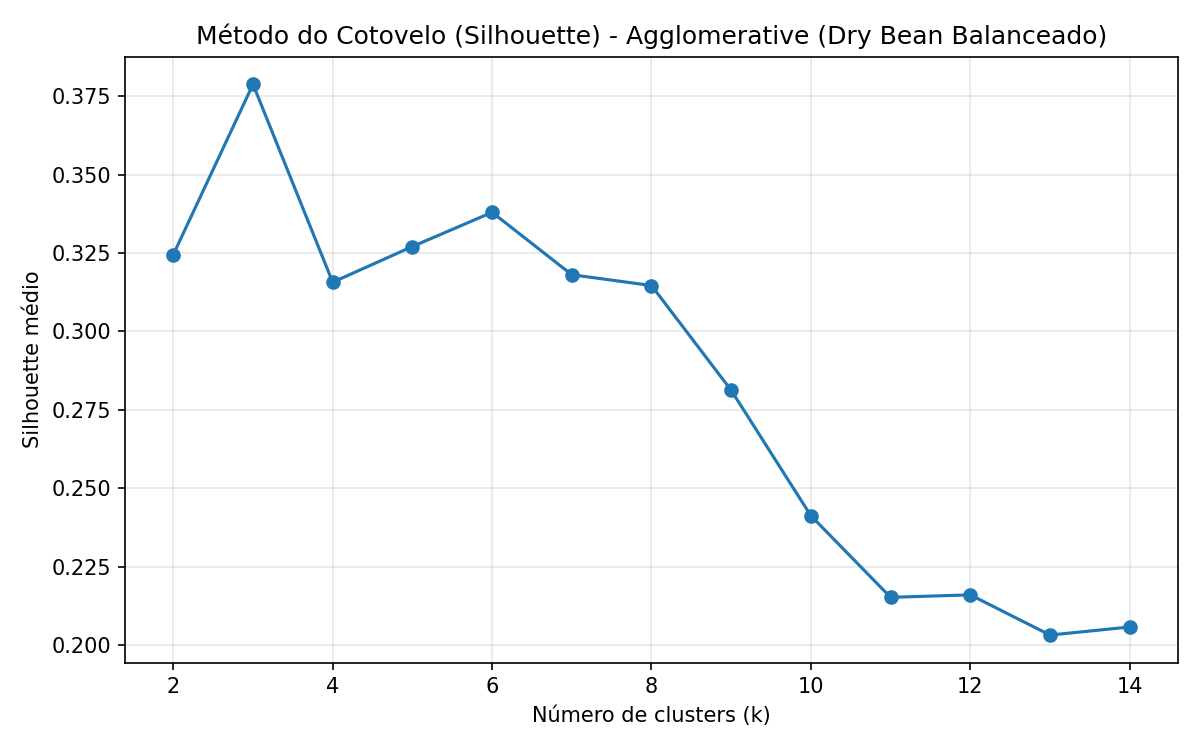
\includegraphics[width=0.7\linewidth]{../src/img/agglo_drybean_balance_silhouette.png}
    \caption{Silhouette médio por número de clusters (Agglomerative - Dry Bean Balanceado)}
\end{figure}

\subsubsection{Dry Bean: Amostras e Pré-processamento}

O conjunto Dry Bean possui 13.611 amostras, 16 atributos e 7 classes (tipos de feijão). O pré-processamento incluiu normalização, codificação e balanceamento por oversampling.

\begin{figure}[ht]
    \centering
    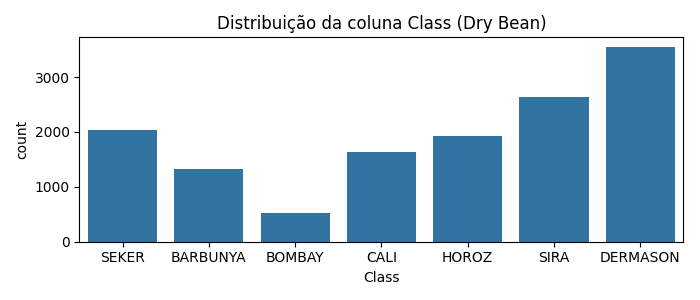
\includegraphics[width=0.7\linewidth]{../src/img/drybean_class_hist_before_balance.png}
    \caption{Distribuição das classes no Dry Bean antes do balanceamento}
    \label{fig:drybean_hist_before_balance}
\end{figure}

\begin{figure}[ht]
    \centering
    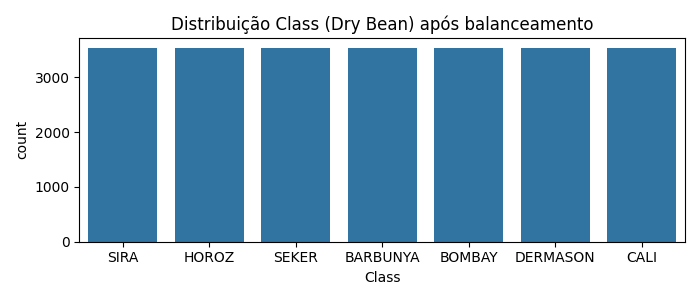
\includegraphics[width=0.7\linewidth]{../src/img/drybean_class_hist_after_balance.png}
    \caption{Distribuição das classes no Dry Bean após o balanceamento}
    \label{fig:drybean_hist_after_balance}
\end{figure}
